\documentclass[a4paper,12pt]{proc}

\usepackage[margin=.5in]{geometry}  
\usepackage[portuguese]{babel} 
\usepackage{multirow}
\usepackage{graphicx}
\usepackage{caption}
\usepackage{subcaption}
\usepackage{mwe}
\usepackage{amsmath}
\usepackage{verbatim}
\usepackage{amssymb}
\usepackage{setspace}

%\singlespacing Para um espaçamento simples
%\onehalfspacing Para um espaçamento de 1,5
%\doublespacing Para um espaçamento duplo

\graphicspath{{images/}}

\title{Relatório Experimento 03:}
\author{Bruno C. Messias}
\date{Julho 2020}

\begin{document}

\maketitle

\section{Introdução}

Este relatório é referente ao experimento 03 da matéria EEL7319(Circuitos RF), sobre o tema de Adaptatação de Impedâncias, que possui o objetivo de avaliar o comportamento dos componentes em aplicações de RF.
Primeiramente foi  calculado os valores teóricos para a adaptção de uma fonte proposta com um eficiência de potência definida, utlizando os conceitos da referência\cite{Orfanidis2003}.
Esse modelo foi testado primeiramente no Software \textit{SimSmith} e implementado no \textit{QUCS} para uma análise mais detalhada. Foi analisado a resposta em frequência da rede de adaptação em ganho e fase. Também foi analisado o potência em cada parte de circuito proposto  

\section{Parte Experimental}

\subsection{Rede de Adaptação}

\subsubsection{Requisitos do Projeto}

Para o projeto inicilamente encontramos a Impedância relativa para a eficiencia requerida de $75\%$ para uma impedância de: \[Z_{S} = (8.5~-~j15)\Omega\]

\noindent Sabemos que a eficiência é definidada pela equação~\ref{eqn1:1} onde $P$ pode ser definida pela equação~\ref{eqn1:2}.

\begin{subequations}
    \label{eqn1}
    \begin{equation}
        \label{eqn1:1}
        \eta = \frac{P_{L}}{P_{S}}
    \end{equation}

    \begin{equation}
        \label{eqn1:2}
        P = 1/2~\Re \left \{ VI^{\ast } \right \}
    \end{equation}

\end{subequations}

\noindent Se utilizando das Equações~\ref{eqn1} chegamos na seguinte expressão, que foi deduzida na seção de Questões deste relatório, na Expressão \ref{eqn-z}.

\[\eta = \frac{\Re\left \{ Y_{x} \right \}}{\Re\left \{ Y_{x} + Y_{s} \right \}} ~~ Onde: Z = \frac{1}{Y}\]

\begin{comment}

\[\eta = \frac{\Re \left \{ Y_{x}\right \}\Re \left \{Y_{x}+Y_{s}\right \}}{\left\lVert Y_{x} + Y_{s}\right\rVert } ~~ Onde: Z = \frac{1}{Y}\]


\noindent Considerando a máxima tranferência onde
$\Im \left \{ Y_{z} \right \}  = - \Im \left \{ Y_{s} \right \}$, temos então a Expressão \ref{max_tranf}.

\begin{equation}
    \eta = \frac{\Re\left \{Y_{x}\right\}}{\Re\left \{ Y_{x} + Y_{s} \right \}}
    \label{max_tranf}
\end{equation}
\end{comment}

\noindent Definimos assim um $Z_{x}$ da qual será nossa referência para a adaptação da impedância de $50~\Omega$. Substituindo os valores obtemos: 
\[Z_{x} =  (8.796~+~j5.223)\Omega \]

\subsubsection{Projeto}

Para definirmos a topologia da rede de adaptação, utilizamos as esquações encontradas na referência\cite{Orfanidis2003}.
Da qual fornece as condições de existência, no nosso caso como temos:

\[R_{G}<R_{L}~e~\left\lvert X_{G} \right\rvert <\sqrt{R_{G}(R_{L}-R_{G})}\] 

\noindent Para esta condição foi escolhida a topologia representada pela Figura~\ref{topo}.

\begin{figure}[htbp]
    \centering
    \includegraphics[scale=.75]{topologia.png}
    \caption{Topologia utilizada para o projeto da rede}
    \label{topo}
\end{figure}

\noindent Seguindo o livro\cite{Orfanidis2003}. 
Para esta topologia temos as equações representadas nas Equações~\ref{eqn3}.

\begin{subequations}
    \label{eqn3}
    \begin{equation}
        \label{eqn3:1}
        X_{1} = \frac{X_{L}\pm R_{L}Q}{\frac{R_{L}}{R_{G}}-1} 
    \end{equation}

    \begin{equation}
        \label{eqn3:2}
        X_{2} = -(X_{G}\pm R_{G}Q)
    \end{equation}

    \begin{equation}
        \label{eqn3:3}
        Q = \sqrt{\frac{R_{L}}{R_{G}}-1+\frac{X_{L}^{2}}{R_{G}R_{L}}}
    \end{equation}

\end{subequations}

\singlespacing

\noindent Assim obtemos os seguintes valores:

\[X_{1} = X_{L} = 23.06 ~e~ X_{2} = X_{C} = -24.22\]

\noindent Portanto assim podemos determinar os componentes pelas seguintes equações:

\begin{subequations}
    \label{eqn4}
    \begin{equation}
        \label{eqn4:1}
        L = \frac{X_{L}}{2\pi f_{0}} 
    \end{equation}

    \begin{equation}
        \label{eqn4:2}
        C = \frac{1}{2\pi f_{0}\left\lvert X_{C}\right\rvert}
    \end{equation}

\end{subequations}

\noindent Para $f_{0} = 5 GHz$ temos os seguintes valores da rede de adpatação representado pela Figura~\ref{topo2}.

\[L = 734.02pH ~e~ C = 1.31pF \]

\begin{figure}[htbp]
    \centering
    \includegraphics[scale=.75]{topologia2.png}
    \caption{Rede a ser utilizada para a adpatação}
    \label{topo2}
\end{figure}

\subsubsection{Análise da Rede}

 Para testar a veracidade dos valores obtidos, foi utilizado como apoio o Software \textit{SimSmith} onde podemos observar o circuito simulado na Figura~\ref{MatchSim} e o resultado na Carta de Smith na Figura~\ref{smith}.

\begin{figure}[htbp]
    \centering
    \includegraphics[scale=.5]{Circuit_Match.png}
    \caption{Circuito Simulado no SimSmith}
    \label{MatchSim}
\end{figure}

\begin{figure}[htbp]
    \centering
    \includegraphics[scale=.2]{Smith_Match.png}
    \caption{Resultado do circuito simulado no SimSmith}
    \label{smith}
\end{figure}

\noindent Podemos observar que o caminho traçado se aproxima do requerido para o projeto com um valor de impedância:
\[Z_{x} =  (8.90~-~j5.41)\Omega \]

\noindent Como mais uma verificação, foi observado a impedância vista da referência, simulado no simulador \textit{Qucs}, representado na Figura~\ref{z}.

\begin{figure}[htbp]
    \centering
    \includegraphics[scale=.5]{impedancia_match.png}
    \caption{Impedância da rede de adpatação}
    \label{z}
\end{figure}

\noindent Onde podemos observar que a sua impedância em $5~GHz$ se equivale a:
\[Z_{x} =  (8.83~-~j5.13)\Omega \]

\noindent Da qual está próximo do valor projetado anteriormente.

\subsubsection{Resposta em frequência}  

Para as seguintes análises foi simulado o modelo proposto no Software \textit{Qucs}, para assim pudermos determinar sua resposta em frequência representados nas Figura~\ref{freq}.

\begin{figure}[htbp]
    \centering
    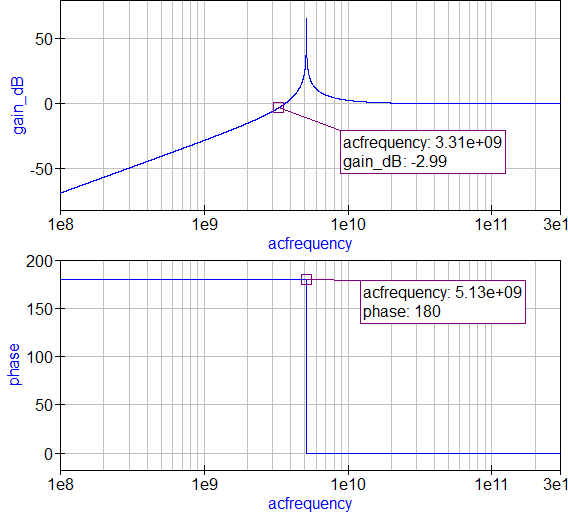
\includegraphics[scale=.5]{Frequency_Response.png}
    \caption{Resposta em frequência da Rede}
    \label{freq}
\end{figure}

\noindent Onde podemos observar um filtro passa-altas com sua freqência de corte próxima de $3.31~GHz$.

\subsubsection{Utilização da Rede}

Para averiguarmos a utilização da rede de adaptação, iremos simular o circuito sem a adaptação primeiramente, forçando $Z_{L}$ para um rendimento de $75\%$, afim de determinarmos os seguintes parâmetros:

\begin{itemize}
    \item Potência da Fonte(Ps)
    \item Potência Disponível(Pd)
    \item Potência na Carga(Pl)
    \item Eficiência(n)
\end{itemize}

\noindent Temos eles representados na Figura\ref{pot}, onde observamos o seu rendimento(n) de $75\%$.

\begin{figure}[htbp]
    \centering
    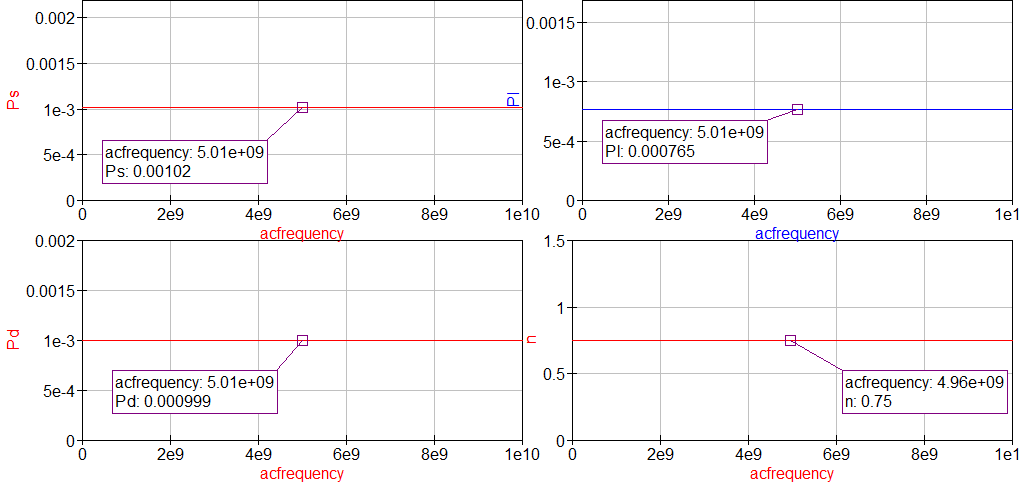
\includegraphics[scale=.33]{Potencias.png}
    \caption{Parâmetros de potência obtidos sem Match}
    \label{pot}
\end{figure}

\noindent Para uma análise de quanto um variação nos componentes pode acarretar va variação das potência e sua eficiência, foi analizado de duas formas: fixando o valor ótimo da parte real de $Z_{L}$ e variando sua parte imaginária representado na Figura~\ref{pot_l_sem} e variando sua parte real com a parte imáginária fixa no valor ótimo, representado na Figura~\ref{pot_r_sem}.

\begin{figure}[htbp]
    \centering
    \includegraphics[scale=.35]{pot_L_sem_match.png}
    \caption{Variação com a varredura da parte imaginária}
    \label{pot_l_sem}
\end{figure}

\begin{figure}[htbp]
    \centering
    \includegraphics[scale=.35]{pot_R_sem_match.png}
    \caption{Variação com a varredura da parte real}
    \label{pot_r_sem}
\end{figure}

\singlespacing

\noindent Podemos observar que ao variar a parte real temos uma maior varição de valores seguindo de acordo com a Equação \ref{eqn-z}, onde o rendimento não depende das componentes imaginárias do circuito.

\singlespacing

\begin{comment}

\noindent Quando variamos a parte imaginária, a varição da eficiência segue a Equação \ref{eqn-z} onde a parte imaginária das impedância ainde tem influência, no entando, não tanto quanto a parte real.
\end{comment}

%\singlespacing

\noindent Incluindo a rede de adpatação temos as seguintes curvas de potência na Figura~\ref{pot_match}.

\singlespacing

\begin{figure}[htbp]
    \centering
    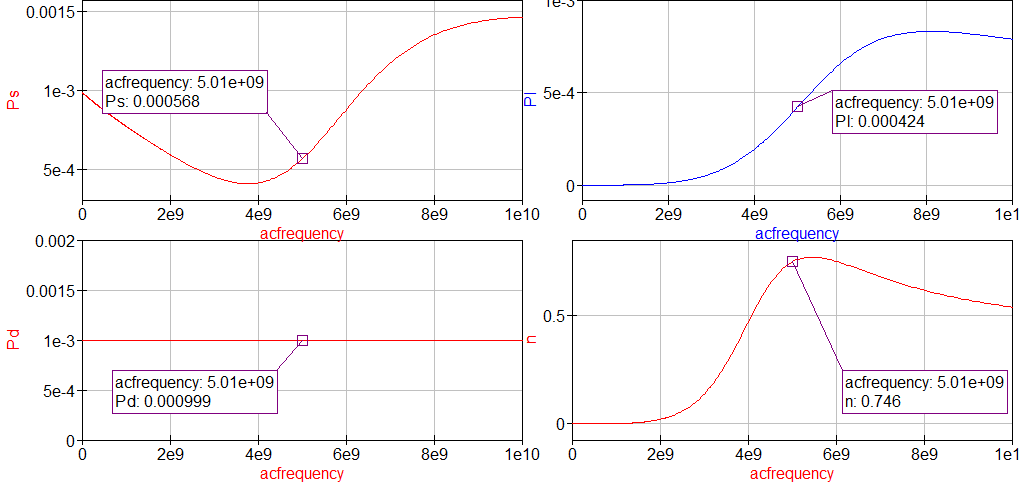
\includegraphics[scale=.33]{Potencia_match.png}
    \caption{Parâmetros de potência obtidos com Match}
    \label{pot_match}
\end{figure}

\noindent Onde podemos analisar que o rendimento manteve-se como esperado do projeto da rede de adaptação.

\singlespacing

\noindent Fazendo a mesma análise feito anteriormente, fixamos sua parte real e fazemos uma vardura na parte imaginária, representado na Figura~\ref{pot_l_com} e fixando a parte imaginária na Figura~\ref{pot_r_com}.

\begin{figure}[htbp]
    \centering
    \includegraphics[scale=.35]{pot_L_com_match.png}
    \caption{Variação com a varredura da parte complexa, considerando a rede}
    \label{pot_l_com}
\end{figure}

\begin{figure}[htbp]
    \centering
    \includegraphics[scale=.35]{pot_R_com_match.png}
    \caption{Variação com a varredura da parte real, considerando a rede}
    \label{pot_r_com}
\end{figure}

\noindent Vemos como a rede de adaptação é bem robusta para a variação da parte imáginária onde o rendimente se manteve sem variação significativa, pois novamente segue de acordo com a Expressão \ref{eqn-z}, da qual não depende de elementos reativos em sua impedância, no entanto ele continua sendo bem suscetível à variações da parte real, como esperado.


\subsection{Componentes Comerciais}

\subsubsection{Modelos Comercias}
Nesta seção iremos substituir os componentes por modelos reais e analisar seu funcionamento quanto as tolerâncias.

\noindent Para o capacitor foi escolido o componente \textmd{C0402C0G1C1R5C020BC} de valor $1.5pF$ da fabricante $TDK^{\copyright}$, que pode ser representado pelo modelo representado na Figura~\ref{cap_model}, com tolerância de $\pm 0.25pF$.

\singlespacing

\noindent E para o indutor, foi escolhido o componente \textmd{MHQ0402PSA0N7BT000} de valor $0.7 nH$, também da mesma fabricante anterior, onde seu modelo pode ser representado pela Figura~\ref{ind_model}, onde possui um tolerância de $\pm 0.1nH$.


\begin{figure}[htbp]
    \centering
    \includegraphics[scale=.5]{modelo_capacitor.png}
    \caption{Modelo comercial do capacitor utilizado}
    \label{cap_model}
\end{figure}

\begin{figure}[htbp]
    \centering
    \includegraphics[scale=.5]{modelo_indutor.png}
    \caption{Modelo comercial do indutor utilizado}
    \label{ind_model}
\end{figure}

\subsubsection{Verificação da Rede}

\noindent Foi verificado com os arquivos Touchstone oferecidos peloa $TDK^{\copyright}$ no software \textit{SimSmith} quanto a sua discrepância ao ser comparado com o modelo teórico, com seu resultado representado a Figura \ref{smith_comercial}.

\begin{figure}[htbp]
    \centering
    \includegraphics[scale=.2]{Smith_Comercial.png}
    \caption{Ábaco de Smith para os modelos comerciais}
    \label{smith_comercial}
\end{figure}

\noindent Podemos observar que a rede faz a tranformação par um valor de $Z =8.38 +j7.77$ que está diferente do requerido por conta das imperfeições introduzidas.

\singlespacing

\noindent Como uma segunda aproximação foi simulado no software \textit{QUCS} a impedância do modelo representado na Figura \ref{z_comercial}.

\singlespacing

\begin{figure}[htbp]
    \centering
    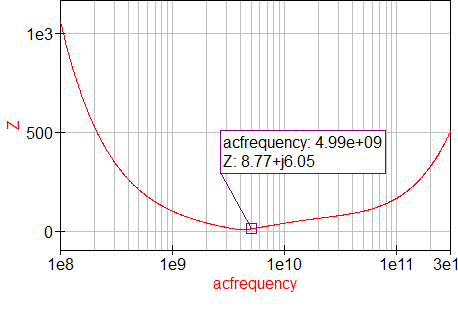
\includegraphics[scale=.5]{z_comercial.png}
    \caption{Impedância da Rede com valores Comerciais}
    \label{z_comercial}
\end{figure}

\noindent Onde chegamos a um valor de $Z = 8.77+j6.05$ próximo do teórico proposto.

\subsubsection{Resposta em freqûencia do modelo}

\noindent Também foi a analizado a resposta em freqência da rede onde podemos observar na Figura \ref{resp_comercial}.

\singlespacing

\begin{figure}[htbp]
    \centering
    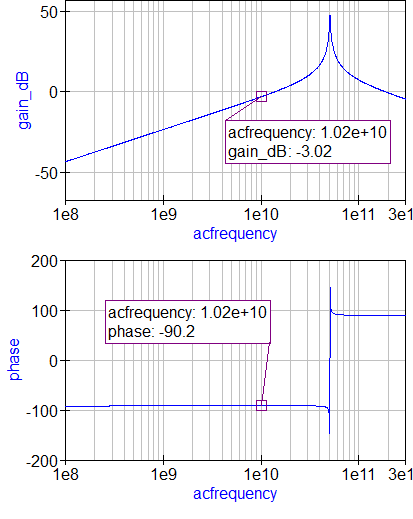
\includegraphics[scale=.5]{resp_comercial.png}
    \caption{Resposta em frequência do modelo comercial}
    \label{resp_comercial}
\end{figure}

\noindent Temos que o circuito de match se comporta como um passa-altas, com frequência de corte próximo de $10.2 GHz$.

\subsubsection{Análise de potência}

Foi analizado a curvas de potencia do circuito com os modelos comerciais que estão representado no Figura \ref{pot_comercial}.

\singlespacing

\begin{figure}[htbp]
    \centering
    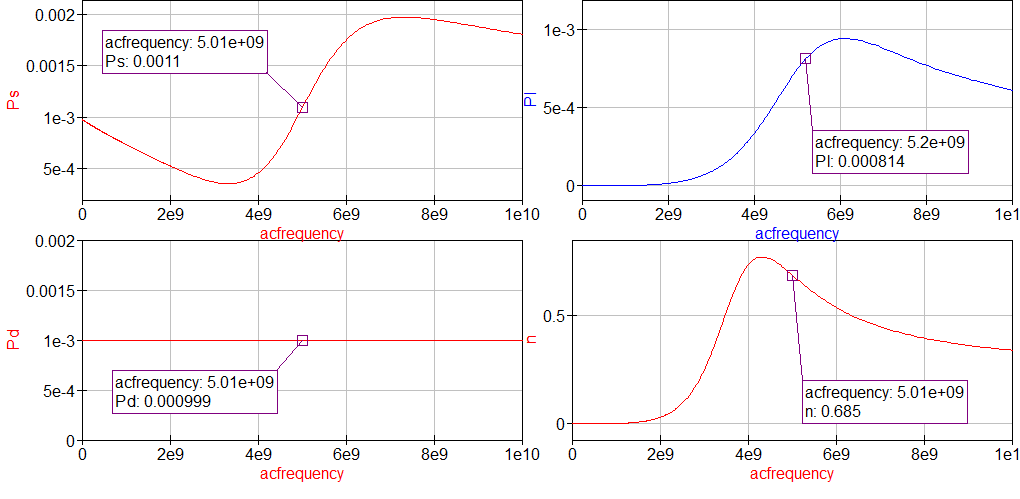
\includegraphics[scale=.30]{potencia_comercial.png}
    \caption{Análise de Potência do modelo comercial}
    \label{pot_comercial}
\end{figure}

\noindent Onde podemos observar sua eficiencia de $\eta=68.5\%$ que difere do proposto anteriormente, por conta das imperfeições introduzidas.

\singlespacing

\noindent Também como feito, como no modelo teórico, variarmos a parte real e fixando a parte imaginária de $Z_{L}$ representada na Figura \ref{R_comercial} e fixando a parte real e variando a imaginária na Figura \ref{L_comercial}

\singlespacing

\begin{figure}[htbp]
    \centering
    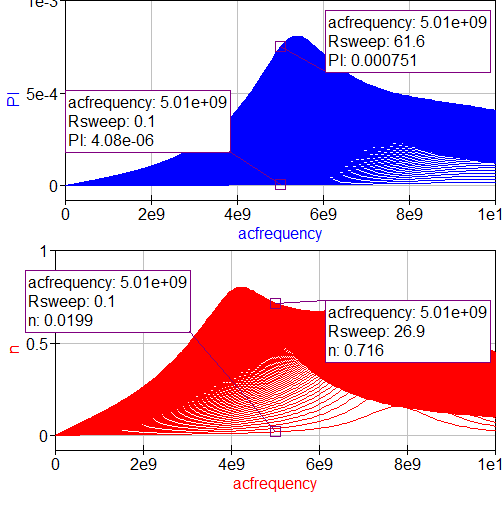
\includegraphics[scale=.5]{pot_R_comercial.png}
    \caption{Varredura na Parte Real}
    \label{R_comercial}
\end{figure}

\begin{figure}[htbp]
    \centering
    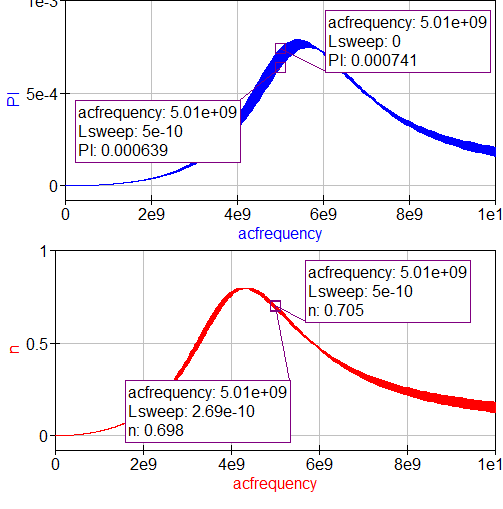
\includegraphics[scale=.5]{pot_L_comercial.png}
    \caption{Varredura na Parte Imaginária}
    \label{L_comercial}
\end{figure}

\noindent Onde podemos comprovar, novamente o analisado anteriormente, pois a variação da parte imaginária não altera o resultado significamente, enquanto a parte real consegue geram grande variações na potência de carga e seu rendimento. 

\subsubsection{Efeito das tolerância}

Utilizando a simulação de Monte Carlo para efeito de observação das tolerâncias fornecidas pelo fabricante, temos as curvas de potência representados na Figura \ref{mont_pot}

\begin{figure}[htbp]
    \centering
    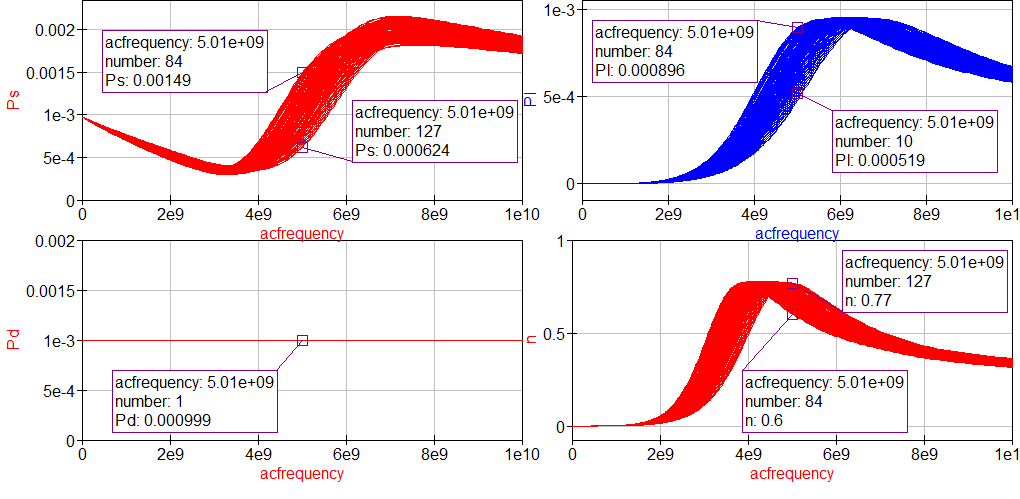
\includegraphics[scale=.3]{mont_potencia.png}
    \caption{Inclusão das tolerância
    especificadas}
    \label{mont_pot}
\end{figure}

\singlespacing

\noindent Temos a seguir os histogramas das simulações de potência da fonte, Figura \ref{hist_ps}, da potência na carga, Figura \ref{hist_pl} e da eficiência na Figura \ref{hist_n}, baseados na simulação de Monte Carlo anterior, desenvolvidos uilizando a linguagem \textit{Python} como apoio.

\begin{figure}[htbp]
    \centering
    \includegraphics[scale=.5]{hist_ps.png}
    \caption{Histograma da Potência da Fonte}
    \label{hist_ps}
\end{figure}

\begin{figure}[htbp]
    \centering
    \includegraphics[scale=.5]{hist_pl.png}
    \caption{Histograma da Potência na Carga}
    \label{hist_pl}
\end{figure}

\begin{figure}[htbp]
    \centering
    \includegraphics[scale=.5]{hist_n.png}
    \caption{Histograma da Eficiência}
    \label{hist_n}
\end{figure}

\noindent Podemos observar que mesmo incluindo as tolerâncias dos elementos da rede de adpatação, o projeto manteve sua eficiência próxima do proposto, com maior incidência ente $75\%$ e $80\%$. 

\section{Sugestão de Melhoria}

\noindent Visto os problemas causados pela adição das não-idealidades dos componentes comerciais, a seguir proponho um modelo que possa aumentar a robustez do projeto contra essas variações.

\singlespacing

\noindent Como sugestão, proponho o uso de duas redes L em cascata como substituição, utilizando o menor Q possível para pudermos analizar seu efeito, toda a documentação de como projetar a rede em cascata está na seção de Questões. 

\singlespacing

\noindent Para o desenvolvimento da rede em cascata, criamos uma impedância virtual que será o terceiro grau de liberdade, segundo o Livro \cite{Orfanidis2003}, o maior R intermediário é encontrado seguindo a Equação, considerando um fator Q mínimo:
\[R = \sqrt{R_{G}R_{L}} \]

\noindent Sabendo que $Z_{G} = 8.796 + j5.223$ e $Z_{L} = 50$, temos que $R = 20.97 \Omega$

\singlespacing

\noindent Temos então a seguinte rede, desenvolvidad como na seção de Questões, representada na Figura \ref{rede_cascade}.

\begin{figure}[htbp]
    \centering
    \includegraphics[scale=.5]{schematic_cascade.png}
    \caption{Rede L em cascata desenvolvida}
    \label{rede_cascade}
\end{figure}

\noindent A partir desta topologia escolhemos componentes comerciais para analizar o efeito das não-idealiades. Foram escolhidos compeonentes da Fabricante $TDK^{\copyright}$ com as seguintes características:

\begin{itemize}
    \item Capacitor de $2pF \pm 0.25pF$; $\rightarrow$Modelo:~\textmd{C0402C0G1C020C020BC}
    \item Capacitor de $1.5pF \pm 0.25pF$, $\rightarrow$Modelo:~\textmd{C0402C0G1C1R5C020BC}
    \item Indutor de $0.5nH \pm 0.1nH$, $\rightarrow$Modelo:~\textmd{MHQ0402PSA0N5BT000}
    \item Indutor de $1.4nH \pm 0.1nH$, $\rightarrow$Modelo:~\textmd{MHQ0402PSA1N4BT000}
\end{itemize}

\noindent Temos a seguir os modelos nas Figuras \ref{cap1}, \ref{cap2}, \ref{ind1} e \ref{ind2}.

\begin{figure}[htbp]
    \centering
    \includegraphics[scale=.5]{modelo_capacitor2.png}
    \caption{Modelo do Capacitor 2pF}
    \label{cap1}
\end{figure}

\begin{figure}[htbp]
    \centering
    \includegraphics[scale=.5]{modelo_capacitor.png}
    \caption{Modelo do Capacitor 1.5pF}
    \label{cap2}
\end{figure}

\begin{figure}[htbp]
    \centering
    \includegraphics[scale=.5]{modelo_indutor1.png}
    \caption{Modelo do Indutor 0.5nH}
    \label{ind1}
\end{figure}

\begin{figure}[htbp]
    \centering
    \includegraphics[scale=.5]{modelo_indutor2.png}
    \caption{Modelo do Indutor 1.4nH}
    \label{ind2}
\end{figure}

\noindent A seguir a análise de potências, sem incluir as tolerâncias num primeiro momento, na Figura \ref{pot_cascade}

\singlespacing

\begin{figure}[htbp]
    \centering
    \includegraphics[scale=.35]{potencia_cascade.png}
    \caption{Análise de Potência na Rede em cascata}
    \label{pot_cascade}
\end{figure}

\noindent Observamos a eficiência próxima de $70.6\%$, já melhor que a rede L original, por conta da inserção dos componentes comerciais e suas não-idealidades.

\singlespacing

\noindent Temos a simulação, considernado o efeito das tolerâncias na Figura \ref{mont_cascade}

\begin{figure}[htbp]
    \centering
    \includegraphics[scale=.35]{mont_cascade.png}
    \caption{Análise de Potência na Rede em cascata considerando tolerâncias}
    \label{mont_cascade}
\end{figure}

\noindent Já observamos uma melhora significativa de quando comparado com a rede L originalmente projetada, pois em consideração a eficiência, temos uma variação de $10.6\%$ e anteriormente, na rede L original, uma variação de $17.6\%$, lembramos que o projeto foi feito para o menor Q possível de ser utilizado, caso utilizássemos um Q maior, observaríamos uma melhora ainda maior em sua robustez quanto as tolerâncias dos componentes.

\section{Questões}

\subsection{Questão 1:}

Para o circuito da figura do experimento, encontre uma expressão para a eficiência de transferência de potência entre fonte
e carga, definida como: 
\[\eta = \frac{P_{L}}{P_{S}}\]
Onde $P_{L}$ é a potência dissipada pela carga e $P_{S}$ é a potência total produzida pela fonte.

\singlespacing

\textbf{Resolução:}

\noindent Sabemos que P é definido pela Equação \ref{eqn1:2}, portanto subistituindo na Equação \ref{eqn1:1} temos:

\begin{equation}
    \eta = \frac{\Re \left \{ V_{x}I_{x}^{\ast } \right \}}{\Re \left \{ V_{s}I_{s}^{\ast } \right \}}
    \label{eqn6}
\end{equation}

\noindent Temos a Figura \ref{circuito_teorico} do circuito a ser analizado.

\begin{figure}[htbp]
    \centering
    \includegraphics[scale=.75]{Pavs_teorico.png}
    \caption{Modelo do circuito a ser analizado para a potência teória}
    \label{circuito_teorico}
\end{figure}

\noindent Sabemos que $V_{x} = V_{s}$ e que $Y=1/Z$ e temos as Equações~\ref{eqn5}.

\begin{subequations}
    \label{eqn5}
    \begin{equation}
        \label{eqn5:1}
        V_{x}= \frac{I_{x}}{Y_{x}}
    \end{equation}

    \begin{equation}
        \label{eqn5:2}
        V_{s}= \frac{I_{s}}{Y_{x}+Y_{s}}
    \end{equation}
\end{subequations}

\noindent Igualando as Equações~\ref{eqn5:1} e \ref{eqn5:2}, temos que:
\[I_{x} = I_{s}\frac{Y_{x}}{Y_{x}+Y_{s}}\]

\noindent Substituindo na Equação \ref{eqn6}, temos que:

\begin{equation}
    \eta = \frac{\Re\left \{ Y_{x} \right \}}{\Re\left \{ Y_{x} + Y_{s} \right \}}
    \label{eqn-z}
\end{equation}

\subsection{Questão 2:}

\noindent Para o circuito da figura do experimento, encontre uma expressão para a eficiência de transferência de potência entre fonte e a carga, definida como:

\[\eta = \frac{P_{L}}{P_{AVS}}\]

\noindent Onde $P_{AVS}$ é a potência disponível da fonte.

\singlespacing

\textbf{Resolução:}

\noindent Para determinarmos $P_{AVS}$ utilizamos a definição da Expressão \ref{eqn1:2}, para a condição de que $ Z_{x} = Z_{s}^{\ast}$, onde temos o circuito a ser analizado na Figura\ref{circuito_teorico}. Temos as seguintes expressões:

\begin{subequations}
    \label{pavs}

    \begin{equation}
        V_{s} =\frac{I_{s}}{Y_{s}+Y_{x}}
    \label{pavs:1}
    \end{equation}

    \begin{equation}
        I_{x} = \frac{I_{s}Y_{s}}{Y_{x} + Y_{s}}
    \label{pavs:2}
    \end{equation}

\end{subequations}

\noindent Utilizando estas definições encontramos que :

\begin{equation}
    P_{AVS} = \frac{I_{s}^{2}}{8 \Re\left \{ Y_{s} \right \}}
    \label{pavs_teo}
\end{equation}

\noindent Inserindo a Expressão \ref{pavs_teo} na definição de $\eta$, temos que:

\begin{equation}
    \eta = \frac{4\Re\left \{ Y_{x}\right \}\Re\left \{ Y_{s} \right \}}{\left \| Y_{s} + Y_{x} \right \|}
    \label{etapavs}
\end{equation}

\subsection{Questão 3:}

Encontre uma expressão para a relação entre a impedância da carga e a impedância da fonte para um determinado valor de
eficiência de transferência de potência e de potência na carga, considerando as duas definições de eficiência, de acordo com
os itens 1 e 2 para o caso onde ambas as impedâncias são complexas.

\singlespacing

\textbf{Resolução:}

\singlespacing

\noindent Temos as seguir os dois gráficos, utilizando as equações encontradas pelas questões anteriores. A definição $\eta = \frac
{P_{L}}{P_{S}}$ representada na Figura \ref{ps_teo} e a definição $\eta = \frac{P_{L}}{P_{AVS}}$ Pela Figura \ref{pavs_teo}, para observarmos como as eficiências se comportam com a variação entre as impedâncias.


\begin{figure}[htbp]
    \centering
    \includegraphics[scale=.5]{eficiencia_n1.png}
    \caption{Eficiência Definida por Pl/Ps}
    \label{ps_teo}
\end{figure}

\begin{figure}[htbp]
    \centering
    \includegraphics[scale=.5]{eficiencia_n2.png}
    \caption{Eficiência Definida por Pl/Pavs}
    \label{pavs_teo}
\end{figure}


\subsection{Questão 4:}
Substitua a rede L utilizada no experimento por uma rede T, de modo a ter uma banda passante de $10\%$.

\singlespacing

\textbf{Resolução:}

\singlespacing

\noindent Para o projeto da rede $T$ vamos seguir a metodologia do livro \cite{Orfanidis2003} onde iremos projetar duas redes L em cascata e combinar elas para um rede $\Pi$ e então transformar em uma rede $T$.

\singlespacing

\noindent Para projetar duas redes L em cascata, primeiramente definimos uma impedância intermediária que define a banda de passagem de $10\%$, para isso definimos $Q = \frac{f_{0}}{BW}$, onde BW é definido como $10\%f_{0}$, para $f_{0} = 5 GHz$, temos então definido $Q = 10$.

\singlespacing

\noindent Para um $Z_{n} = R + jX $ intermediário, temos que R é definido pela Expressão \ref{Rn}, retirado do livro \cite{Orfanidis2003}.

\begin{equation}
    R = \frac{R_{max}}{Q^{2}+1}~~Onde:R_{max} = (R_{G},R_{L})
    \label{Rn}
\end{equation}

Sabemos que $ Z_{G} = 5 \Omega$ e $Z_{L} = 8.796 + j5.223 \Omega $, com essas informações e a Equação \ref{Rn}, temos $R = 0.49 \Omega$, como a parte imaginária é arbitrária escolhemos $X = 0 $ e logo temos $Z = 0.49$.

\subsubsection{Projeto Primeira rede L}

Temos o projeto da primerira rede L considerando $Z_{L} = 50 \Omega$ e $Z_{G} = 0.49$, Como $R_{G} < R_{L}$, utilizamos Equações do livro \cite{Orfanidis2003}.

\begin{subequations}
    \label{eqn3_t}
    \begin{equation}
        \label{eqn3_t:1}
        X_{1} = \frac{X_{G}\pm R_{G}Q}{\frac{R_{G}}{R_{L}}-1} 
    \end{equation}

    \begin{equation}
        \label{eqn3_t:2}
        X_{4} = -(X_{L}\pm R_{L}Q)
    \end{equation}

    \begin{equation}
        \label{eqn3_t:3}
        Q = \sqrt{\frac{R_{G}}{R_{L}}-1+\frac{X_{G}^{2}}{R_{G}R_{L}}}
    \end{equation}

\end{subequations}

\noindent Com as Equações \ref{eqn3_t}, definimos:

\[X_{1} = 2.812 ~e~ X_{4} = -2.36\]

\subsubsection{Projeto Segunda rede L}

Temos o projeto considerando $Z_{L} = 0.49$ e $Z_{G} = 8.796 + j5.223 $, Como $R_{G} > R_{L}$, utilizamos as Equações \ref{eqn3} utilizadas anteriormente.

\noindent Utilizando esses dados e a Expressões \ref{eqn3}, temos os seguintes resultados:

\[X_{3} = 4.97 ~e~ X_{5} = -4.925\]

\subsubsection{Projeto Rede T}

\noindent Temos então que $X_{2} = X_{4} + X_{5} = - 7.285$, para uma rede $\Pi$, para converter para uma rede T, utilizamos as  Equações \ref{eqn_T} , retiradas do livro \cite{Orfanidis2003}, para a topologia representada pela Figura~\ref{topologia_T}.

\begin{subequations}
    \label{eqn_T}
    \begin{equation}
        Z_{a} = \frac{Z_{2}Z_{3}}{U}
        \label{eqn_T:1}
    \end{equation}
    \begin{equation}
        Z_{b} = \frac{Z_{3}Z_{1}}{U}
        \label{eqn_T:2}
    \end{equation}
    \begin{equation}
        Z_{c} = \frac{Z_{1}Z_{2}}{U}
        \label{eqn_T:3}
    \end{equation}
    \begin{equation}
        U = Z_{1}+Z_{2}+Z_{3}
        \label{eqn_T:4}
    \end{equation}
\end{subequations}

\begin{figure}[htbp]
    \centering
    \includegraphics[scale=.5]{topologia_T.png}
    \caption{Topologia da rede T}
    \label{topologia_T}
\end{figure}

\noindent Como temos que $Z_{1} = jX_{1}$ e $Z_{2} = jX_{2}$ e $Z_{3} = jX_{4}$, chegamos nos valores de $Z_{a} = j72.85$, $Z_{b} = -j28.12$ e $Z_{c} = j41.22$, onde temos o circuito composto por componentes representado na Figura \ref{schematic_T}.

\begin{figure}[htbp]
    \centering
    \includegraphics[scale=.5]{schematic_T.png}
    \caption{Esquemático da Rede T}
    \label{schematic_T}
\end{figure}

\subsubsection{Análise de Freqûencia da rede T}

Temos a seguir as análises de frequência da rede T na Figura \ref{resp_T}.

\begin{figure}[htbp]
    \centering
    \includegraphics[scale=.5]{resp_T.png}
    \caption{Resposta em frequência da rede T}
    \label{resp_T}
\end{figure}

\noindent Onde podemos observar que a rede se comporta como um filtro passa-baixas com um frequência de corte próximo de $f_{c} = 4.19 GHz$.


\subsubsection{Análise de funcionamento da rede}

Temos a seguir a sua resposta de casamento de impedância gerados pelo software \textit{SimSmith}, utilizando o circuito na Figura \ref{cir_smith_T} e sua carta de smith na Figura \ref{smith_T}.

\begin{figure}[htbp]
    \centering
    \includegraphics[scale = .32]{cir_smith_t.png}
    \caption{Circuito utilizado no Software SimSmith}
    \label{cir_smith_T}
\end{figure}

\begin{figure}[htbp]
    \centering
    \includegraphics[scale=.3]{smith_t.png}
    \caption{Ábaco de Smith gerado}
    \label{smith_T}
\end{figure}

\noindent Vemos que sua tranformação de impedância termina no ponto $Z = 9 + j5.25 \Omega$ que está próximo do esperado de $Z = 8.796 + j5.223 \Omega$.

\singlespacing

\noindent Como uma segunda análise temos a seguir a análise de impedância simulada no software \textit{QUCS}, representada na Figura \ref{Z_T}

\begin{figure}[htbp]
    \centering
    \includegraphics[scale=.5]{Z_T.png}
    \caption{Impedância da rede T simulada}
    \label{Z_T}
\end{figure}

\noindent Onde podemos observar que o circuito aproxima para um $Z = 8.88 - j5.35 \Omega$, bem próximo do proposto.

\subsubsection{Análise de potências da rede T}

Temos a seguir uma análise de potência substituindo a rede L anteriormente projetada pela rede T proposta nessa seção, representadas na Figura \ref{pot_T}.

\begin{figure}[htbp]
    \centering
    \includegraphics[scale =.3]{potencia_T.png}
    \caption{Análise de Potências da rede T}
    \label{pot_T}
\end{figure}

\noindent Onde podemos observar que temos sua eficiência de $74.5\%$ como era esperado pelo projeto.

\singlespacing

\noindent Analizamos seguindo as mesma etapas feitas anteriormente para a rede L, logo temo também suas varreduras na parte imaginária e na parte real, representadas pelas Figuras \ref{imag_t} e \ref{real_t}

\begin{figure}[htbp]
    \centering
    \includegraphics[scale=.5]{pot_L_t.png}
    \caption{Varredura na parte imaginária com a parte real fixa}
    \label{imag_t}
\end{figure}


\begin{figure}[htbp]
    \centering
    \includegraphics[scale=.5]{pot_R_t.png}
    \caption{Varredura na parte real com a parte imaginária fixa}
    \label{real_t}
\end{figure}

\singlespacing

\noindent Como conclusão, a rede T mantém suas mesmas características quando comparadas com a rede L, no entando como temos um maior grau de liberdade podemos dimensionar um circuito mais seletivo em questão de tranferência de potência, que o torna mais robusto em variações dos componentes.

\section{Conclusão}

Em conclusão, este relatório tinha como objetivo, analizar todo o processo de casamento de impedânicas, considerando uma eficiência fixa e máxima tranferência de potência. 

\singlespacing

\noindent Foi analizado e comprovado as equações de eficiência, quando a varreduras em componentes imaginários e reais, fornçãndo um descsamento e seu efeito no análise de potência. 

\singlespacing

\noindent Foi estudado a utilizadção de modelos dipolos no simulador \textit{QUCS}, bem como a utilização de modelos comerciais e análise de possibilidade de utilização do projeto na realidade e como o efeito de tolerância pode afetar na resposta da rede de adpatção. 

\singlespacing

\noindent Foi sugerido melhorias para uma melhor robustez no projeto por conta das não-idealidades dos componentes reais e a utilização de diferentes redes de adptção usando componentes discretos. 

\singlespacing

\noindent E também foi analizado as duas definições de eficiência e de como diferem quando levando em conta o projeto da rede.

\section{Referências}

\nocite{*}

\bibliographystyle{IEEEtran}
\bibliography{Lab_03}


\end{document}